\begin{figure}[htbp]
\section*{ RPGRIP1}
\centering
\begin{subfigure}[b]{0.95\textwidth}
\centering
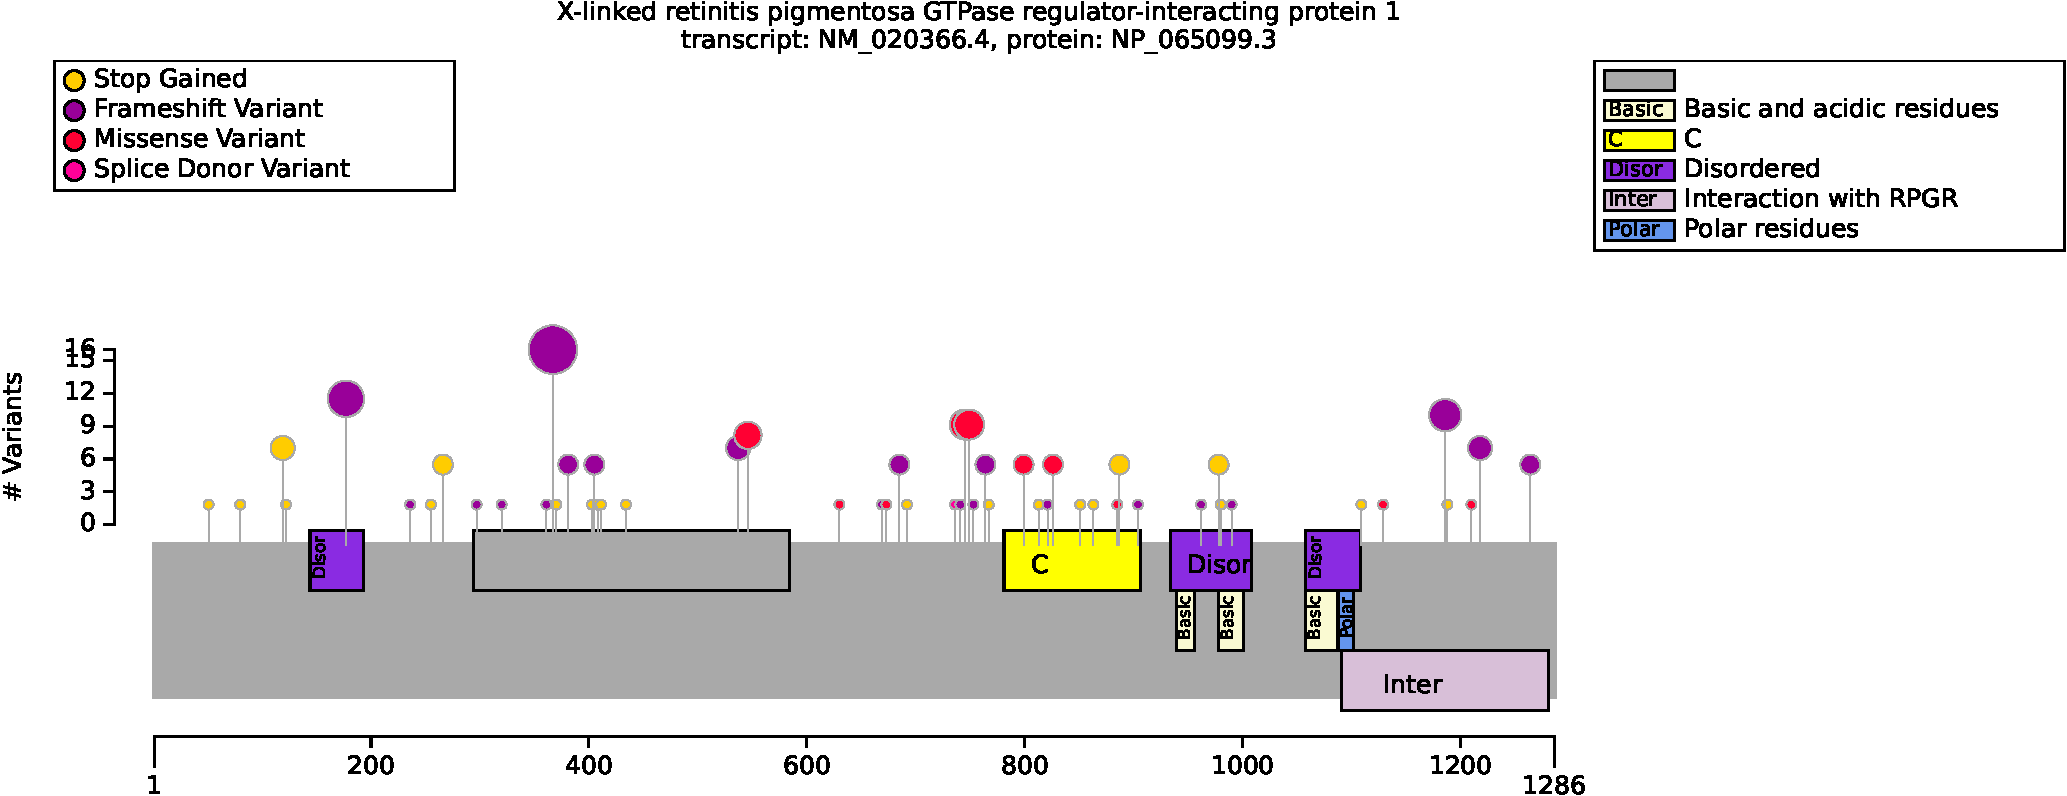
\includegraphics[width=\textwidth]{ img/RPGRIP1_protein_diagram.pdf} 
\captionsetup{justification=raggedright,singlelinecheck=false}
\caption{Distribution of variants in RPGRIP1}
\end{subfigure}

\vspace{1em}

\begin{subfigure}[b]{0.95\textwidth}
\centering
\resizebox{\textwidth}{!}{
\begin{tabular}{llllrr}
\toprule
HPO term & 1107del/1107del OR 1107del/other & other/other & p-value & adj. p-value\\
\midrule
Eye poking [HP:0001483] & 16/16 (100\%) & 19/41 (46\%) & $1.30\times 10^{-4}$ & 0.002\\
\bottomrule
\end{tabular}
}
\captionsetup{justification=raggedright,singlelinecheck=false}
\caption{         Fisher Exact Test performed to compare HPO annotation frequency with respect to 1107del/1107del OR 1107del/other and other/other. Total of
        16 tests were performed. }
\end{subfigure}
\vspace{1em}
\begin{subfigure}[b]{0.95\textwidth}
\centering
\resizebox{\textwidth}{!}{
\begin{tabular}{llllrr}
\toprule
HPO term & OMIM:613826 & OMIM:608194 & p-value & adj. p-value\\
\midrule
Nystagmus [HP:0000639] & 64/66 (97\%) & 11/16 (69\%) & 0.003 & 0.020\\
Very low visual acuity [HP:0032122] & 35/39 (90\%) & 4/16 (25\%) & $5.21\times 10^{-6}$ & $7.81\times 10^{-5}$\\
\bottomrule
\end{tabular}
}
\captionsetup{justification=raggedright,singlelinecheck=false}
\caption{Fisher Exact Test performed to compare HPO annotation frequency with respect to OMIM:613826 and OMIM:608194. Total of
        15 tests were performed. }
\end{subfigure}
\vspace{1em}
\begin{subfigure}[b]{0.95\textwidth}
\centering
\resizebox{\textwidth}{!}{
\begin{tabular}{llllrr}
\toprule
Genotype (A) & Genotype (B) & total tests performed & significant results\\
\midrule
missense/missense & missense/other OR other/other & 17 & 0\\
frameshift/frameshift & frameshift/other OR other/other & 16 & 0\\
FEMALE & MALE & 16 & 0\\
\bottomrule
\end{tabular}
}
\captionsetup{justification=raggedright,singlelinecheck=false}
\caption{             Fisher Exact Test performed to compare HPO annotation frequency with respect to genotypes. }
\end{subfigure}

\vspace{0.2em}

\caption{ The cohort comprised 100 individuals (45 females, 49 males, 6 with unknown sex). A total of 45 HPO terms were used to annotate the cohort. Disease diagnoses: Leber congenital amaurosis 6 (OMIM:613826) (79 individuals), Cone-rod dystrophy 13 (OMIM:608194) (21 individuals). It was reported that Patients with a double null genotype may develop 
symptoms earlier and have worse vision \cite{PMID_38768745}. We did not observe a corresponding significant correlation in our dataset. A total of 71 unique variant alleles were found in \textit{RPGRIP1} (transcript: \texttt{NM\_020366.4}, protein id: \texttt{NP\_065099.3}).}
\end{figure}
